{{\textbf{存储器主要有3个性能指标:速度、容量、价格。}}{一般来说,速度越高,价格就越高;容量越大,价格就越低,而且容量越大,速度必定越低,}}{如下图}{所示。而理想的存储器应该是大容量、高速度、低价格。}

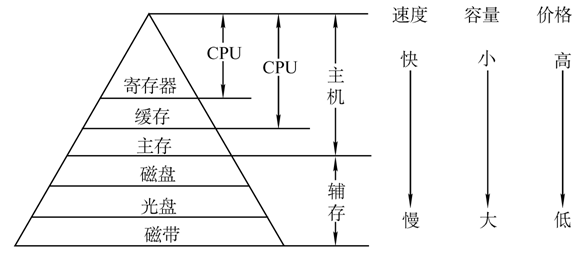
\includegraphics[width=3.69792in,height=1.61458in]{png-jpeg-pics/99E962691CE4528C6959B97044926CC7.png}

\textbf{{存储系统的层次结构}}{主要体现在缓存-主存和主存-辅存这两个存储层次上,如下图所示。显然,CPU和缓存、主存都能直接交换信息;缓存能直接和CPU、主存交换信息;主存可以和CPU、缓存、辅存交换信息。}

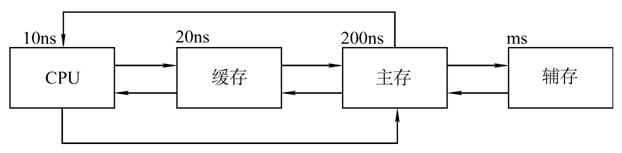
\includegraphics[width=3.69792in,height=0.90625in]{png-jpeg-pics/E1DED16052D8BEF6EFA4905541EAD992.png}

{主存-辅存层次主要解决存储系统的容量问题。主存和辅存之间的数据交换是由硬件和操作系统共同完成的。}
